\begin{figure}
\centering
 \subfloat[][]{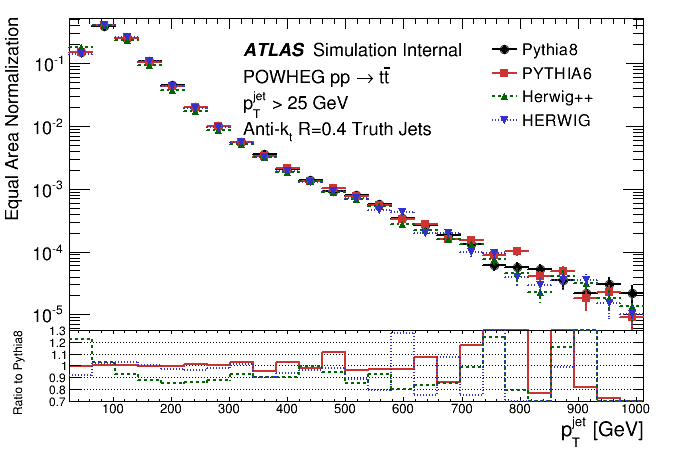
\includegraphics[width=0.45\columnwidth]{evtgen/figures/Frag/Top/SingleB/h_JetpT.png}}
 \subfloat[][]{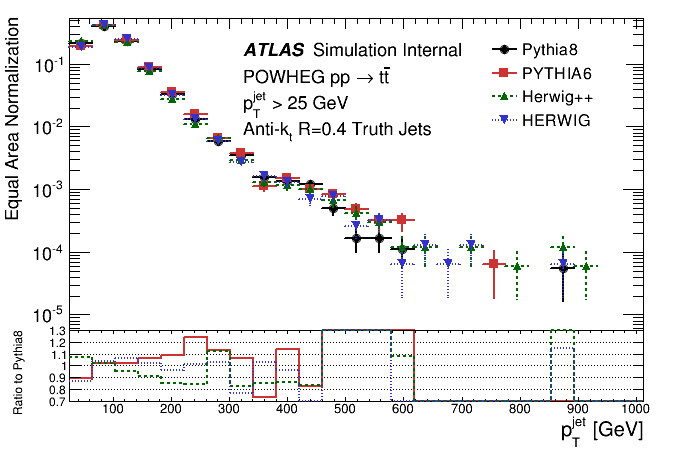
\includegraphics[width=0.45\columnwidth]{evtgen/figures/Frag/Top/SingleC/h_JetpT.png}}
\caption{Comparison of the $p_T$ of (a) b-jets and (b) c-jets in \PythiaE, \Pythia, \Herwigpp, and \Herwig.  \ttbar\ samples. Jets with only a single heavy flavor hadrons are selected, as discussed in Section~\ref{sec:fragmentation}.}
\label{fig:jetpt}
\end{figure}